%Review of existing harmonic excitation.
%	Nonlinear Systems
%		Traditional Metrics (THD, IMD)
%		Minimisation of Nonlinear Distortion
%		Advent of "Nonlinear Niceness"
%	Timbre of nonlinear distortions (Martens and Marui type shit)
%	Uses of Harmonic Excitation
%	Harmonic Generation Methods
%		Static Nonlinearities
%		Bandwidth Extension (high frequency reconstruction)
%		Individual Harmonic Generation (SMC paper)
%		Psychoacoustic Enhancers

\chapter{Harmonic Excitation}
\label{chap:Excitation}

\section{Introduction}
\label{sec:Excitation-Introduction}
	Nonlinear distortion is an inherent part of an analogue signal path. It alters the dynamic variation of signals and
	introduces new spectral components. Its use as a creative effect is best know by guitar players
	\citep{dutilleux2011nonlinear}. This was due to the use of values in early guitar amplifiers imparting nonlinear
	transforms onto the audio signal. This distorted sound became desirable and several electronic circuits were
	developed with the purpose of inducing nonlinear distortion. More recently research into modelling these distortion
	circuits in the digital domain has been carried out, such as that done by \citet{pakarinen2009a}. Several
	researchers have also worked on creating novel digital distortion techniques \citep{fernandez-cid2001distortion,
	pekonen2008coefficient, puckette2007patch}.

	Distortion is a very broad term which is typically used to describe unwanted effects. For this work a better defined
	term, harmonic excitation, will be used to refer to the deliberate and controlled application of nonlinear systems
	in order to introduce new frequency components to a signal. \citet{dutilleux2011nonlinear} defines excitation as
	the process of controlling timbre through the emphasis of certain frequencies. While this is possible with linear
	systems, such as equalisers, nonlinear systems provide more flexibility as they can add energy in areas of the
	spectrum where the original signal had none.

	This chapter will review how nonlinear systems have been analysed in previous audio research, how their effects are
	quantified and the timbral transformations they impart. The current uses of harmonic excitation in audio engineering
	are then discussed in Section \ref{sec:Excitation-Uses}. A list of criteria with which to evaluate harmonic
	excitation methods for use in real time timbral control is developed in Section \ref{sec:Excitation-Evaluation}.
	Section \ref{sec:Excitation-Methods} then describes several methods for harmonic excitation and how they perform in
	these areas.  Issues with certain methods are identified and ways to overcome them suggested.

\section{Analysis of Nonlinear Systems}
\label{sec:Excitation-AnalysisOfNonlinearSystems}
	The analysis of nonlinear system is more complicated that that of linear systems. This is due to more features of
	the input signal affecting how the system responds. In the field of audio engineering much of the literature
	concerning nonlinearities has to do with minimising distortion or measuring the maximum allowable levels of
	distortion. Several distortion metrics have been developed each with there own uses. A review of many of these
	metrics is given by \cite{voishvillo2006assessment}, some of which will be discussed in this section.

	\subsection{Objective Distortion Metrics}
	\label{sec:Excitation-Analysis-Metrics}
		Total Harmonic Distortion (THD) and Intermodulation Distortion (IMD) are the traditional objective measures
		of distortion \citep{czerwinski2001multitone1}. THD measures the level of new frequency components
		introduced by a system which are harmonically related to the original signal.  There are two different ways
		in which THD is calculated. These have been denoted $THD_{F}$ and $THD_{R}$ by \citet{shmilovitz2005on} and
		are calculated using Equations \ref{eq:thdf} and \ref{eq:thdr} respectively.

		\begin{equation}
			THD_{F} = \frac{\sqrt{\sum_{n = 2}^{\infty} A_{n}^{2}}}{A_{1}}
			\label{eq:thdf}
		\end{equation}

		\begin{equation}
			THD_{R} = \sqrt{\frac{\sum_{n = 2}^{\infty} A_{n}^{2}}{\sum_{n = 1}^{\infty} A_{n}^{2}}}
			\label{eq:thdr}
		\end{equation}

		Where $A_n$ is the amplitude of the $n_{th}$ harmonic. 

		Both these methods been used in recent work published in the audio field ($THD_{F}$ by
		\citet{fleischmann2014a} and $THD_{R}$ by \citet{dutilleux2011nonlinear}). The lack of standardisation for
		this metric makes it difficult to compare experiment results reported by different sources.

		IMD is a measure of the new spectral content introduced by a system as a result of intermodulation between
		the frequency components of the original signal. There are several different standards for the calculation
		of IMD some of which are listed by \citet{voishvillo2006assessment}.

		THD and IMD give very limited information about the response of nonlinear systems. They are typically
		measured using simple input signals which are not representative of the signals a system would process in
		actual use. Given that nonlinear systems my not satisfy the condition of superposition a system may process
		simple and complex signals in vastly differing manners. 

		These metrics also give no indication of the perceived degradation in audio quality a system introduces. A
		signal with a high THD values may sound less distorted that one with a small THD. Several researchers have
		developed new distortion metrics which indicate the perceived amount of distortion.

		\citet{geddes2003auditory} suggest some psychoacoustic principles which may be applicable to the analysis of
		nonlinear distortion:

		\begin{itemize}
			\item New frequency components introduced, with lower frequencies that the original components, will
			      be more perceptible.
			\item Higher order nonlinearity artefacts will be more perceptible.
			\item Nonlinearities which affect lower amplitude signals will be more perceptible.
		\end{itemize}

		\citet{voishvillo2006assessment} adds that the perception of distortion is decreased at the very high and
		low ends of the frequency spectrum.

		The GedLee metric, proposed by \citet{geddes2003auditory}, measures how much a nonlinearity will be
		perceived through analysis of its characteristic curve. It is calculated using Equation \ref{eq:gedlee}.

		\begin{equation}
			G_{m} = \sqrt{\int_{-1}^{1} \left( \cos \left( \frac{x\pi}{2} \right) \right)^{2}
				      \left( \frac{d^{2}}{dx^{2}} T(x) \right)^{2} dx}
			\label{eq:gedlee}
		\end{equation}

		Where $T(x)$ is the characteristic curve of the nonlinearity in question.

		A considerable advantage of the GedLee metric is that it directly measures the system in question rather
		than signals processed by it. This should allow measurements taken using the metric to describe the audible
		degradation of any signal processed by a system. \citet{lee2003auditory} provide results of an experiment in
		which their metric was tested against THD and IMD as a rating of audio quality. They show that for low
		levels of distortion the GedLee metric correlates with subjective audio quality ratings. THD and IMD are
		both found to not correlate well with perceived quality.

		In Equation \ref{eq:gedlee} the system being analysed is assumed to be a simple static nonlinearity. Many
		nonlinear systems are more complex than this and may exhibit frequency dependant or time varying behaviour.
		While the GedLee metric may provide a good, signal independent, measure of distortion, it is only applicable
		to a subset of nonlinear systems.

		\citet{tan2003the} also developed a perceptual metric for distortion, Distortion Score (DS), which they then
		improved upon to create the $R_{nonlin}$ metric \citep{tan2004predicting}. Both these metrics rely on
		analysing signals which have been processed so they may not give results which can be applied as generally
		as those using the GedLee metric. Where these metrics have an advantage is that they use models of the human
		hearing system to better approximate the perceived level of distortion.

		To calculate the DS the audio is split into frequency bands which model the auditory filters of the
		cochlear. These auditory filters represent bands in which two tones will interfere with the perception of
		each other \citep{fastl2007psychoacoustics}. Tones can be masked (made inaudible) by other tones within the
		same auditory filter band. By processing the audio in this manner the DS metric can take account of elements
		of the distortion which may not be perceptible because of masking.
		
		The $R_{nonlin}$ metric improves on this model of the hearing system by including a filter with a frequency
		response similar to that of the outer and middle ear. The filter used is as described by
		\citet{glasberg2002a}, it attenuates frequencies at either end of the audible spectrum. This models the
		decreased perception of distortion at these frequencies discussed earlier.

		\citet{tan2004predicting} report greater correlation between $R_{nonlin}$ and perceived audio quality then
		\citet{lee2003auditory} do for the GedLee metric. They also demonstrate how accurate the $R_{nonlin}$ metric
		is in predicting the perceived distortion level introduced to music and speech signals.

		The research discussed in this section has focused on measuring the extent to which unwanted distortion can
		be perceived. This does not provide enough information for the description of timbre. The listening test
		performed to verify the developed metrics asked subjects to rate the quality of audio samples. Nonlinear
		distortion could alter the timbre of audio without deteriorating its perceived quality. It may also be
		possible to describe the timbre of different nonlinear distortions further rather than ranking them on the
		same distortion scale. Research has been carried out into the timbre of distortion as discussed in Section
		\ref{sec:Excitation-Timbre}.

		\subsection{Nonlinear Modelling}
		Various techniques for modelling nonlinear systems have been developed in the mathematics and engineering
		literature. These models allow for more in depth analysis of a system as well as replicating its effects in
		the digital domain. Summaries of some of these modelling techniques can be found in the work by
		\citet{janczak2005identification} and \citet{ogunfunmi2007adaptive}.

		Two nonlinear modelling techniques have found use in audio processing:

		\begin{itemize}
			\item Wave Digital Filters as discussed by \citet{fettweis1986wave}.
			\item The Synchronised Swept Sine Method as described by \citet{novak2010nonlinear}.
		\end{itemize}

		These techniques are summarised here.

		\subsubsection{Wave Digital Filters}
			Wave digital filters are a class of filter which can be used to emulate analogue circuits. The
			process of creating a digital of a circuit involves constructing a `tree' of blocks. These blocks
			represent either electronic components, or connections between components in a circuit. Each block
			obeys a certain set of rules when presented with a signal. Blocks have been developed for modelling
			nonlinear circuit elements such as operational amplifiers and diodes \citep{paiva2012emulation}.

			While wave digital filters can accurately represent a nonlinear system there are some disadvantages.
			As systems get more complex traversing the `tree' of blocks in order to calculate the output signal
			takes more computation. This presents problems when real time system response is needed. There are
			also certain circuit topologies which cannot be represented in the wave digital domain
			\citep{valimaki2011virtual}. Another consideration is that knowledge of the circuitry inside a
			system being modelled is needed. This might not always be available.

		\subsubsection{The Synchronised Swept Sine Method}
			The synchronised swept sine method is a technique for identifying nonlinear systems without prior
			knowledge of their operation. The details of its operation are describe by
			\citet{novak2010nonlinear}. The result of the testing is a series of filter kernels to be used in
			the model shown in Figure \ref{fig:hammerstein}.

			\begin{figure}[h!]
				\centering
				\begin{tikzpicture}
					\node (Sig2) [draw] at (1, 3) {$x^{2}(t)$};
					\node (Sig3) [draw] at (1, 2) {$x^{3}(t)$};
					\node (SigN) [draw] at (1, 0.5) {$x^{N}(t)$};

					\node (Filter1) [draw] at (3, 4) {$A_{1}(f)$};
					\node (Filter2) [draw] at (3, 3) {$A_{2}(f)$};
					\node (Filter3) [draw] at (3, 2) {$A_{3}(f)$};
					\node (FilterN) [draw] at (3, 0.5) {$A_{N}(f)$};

					\draw (Sig2) -- (Filter2);
					\draw (Sig3) -- (Filter3);
					\draw (SigN) -- (FilterN);

					\draw [dots] (Sig3) -- (SigN);
					\draw [dots] (Filter3) -- (FilterN);

					\coordinate (Out1) at (4.5, 4);
					\coordinate (Out2) at (4.5, 3);
					\coordinate (Out3) at (4.5, 2);
					\coordinate (OutN) at (4.5, 0.5);

					\draw (Filter1) -- (Out1);
					\draw (Filter2) -- (Out2);
					\draw (Filter3) -- (Out3);
					\draw (FilterN) -- (OutN);

					\node (Add) [operator] at (5, 2.25) {+};
					\draw (Out1) -- (Add);
					\draw (Out2) -- (Add);
					\draw (Out3) -- (Add);
					\draw (OutN) -- (Add);

					\coordinate (In1) at (-0.5, 4);
					\coordinate (In2) at (-0.5, 3);
					\coordinate (In3) at (-0.5, 2);
					\coordinate (InN) at (-0.5, 0.5);

					\draw (In1) -- (Filter1);
					\draw (In2) -- (Sig2);
					\draw (In3) -- (Sig3);
					\draw (InN) -- (SigN);
					\draw (InN) -- (In1);

					\node (In) at (-1.25, 2.25) {$x(n)$};
					\coordinate (InMid) at (-0.5, 2.25);
					\draw (In) -- (InMid);

					\node (Out) at (6, 2.25) {$y(n)$};
					\draw (Add) -- (Out);

				\end{tikzpicture}
				\caption{Generalised Polynomial Hammerstein Model}
				\label{fig:hammerstein}
			\end{figure}

			The model is, in effect, an extension of a Taylor Series of order $N$. The input is raised to each
			individual power, 1 through $N$, and each of these signals is filtered by an individual kernel,
			$A_{N}(f)$. The resultant signals are then summed to produce the output.

			This method is easier to implement that a wave digital filter as no prior knowledge of the system is
			needed. The amount of computation time needed to process a signal is also considerably less. There
			are however some disadvantages. There is no account for the dependence of the system on the
			amplitude of the input signal. This is shown by \citet{novak2010analysis} who demonstrate how two
			different circuits are emulated with different degrees of accuracy. The is also no definite way of
			deciding what order Hammerstein model to use prior to testing.

\section{Timbre of Nonlinear Distortion}
\label{sec:Excitation-Timbre}
	There is a wealth of research into how low level audio features influence timbre \note{(probably refer to stuff in
	the timbre chapter here)}. The mappings between low level features and semantic features from the literature can be
	applied to harmonic excitation effects provided the excitation method used can influence the required low level
	features. There may be semantic terms used to describe the timbre of nonlinear distortion which are seldom used to
	describe other timbres. The majority of timbral research does not focus on nonlinear distortion and as such does not
	highlight these semantic terms. There have been some publications specifically discussing the timbral effects of
	nonlinear distortion. Their findings are discussed in this section.

	\citet{marui2005predicting} suggest that one of the primary outcomes of nonlinear distortion is the moving
	of spectral energy between low and high frequencies. An effect they propose correlates with the descriptors
	sharpness and brightness. In order to discover other timbral properties of nonlinear distortion they performed
	listening tests in which distorted guitar samples were assessed. The samples were each processed with different
	nonlinear systems and then further processed so that they had matching Zwicker Sharpnesses (an objective measure of
	sharpness \cite{fastl2007psychoacoustics}). This sharpness matching was does so that difference in timbre not
	related to sharpness could be more easily observed. During the listening tests subjects were asked to rate the
	dissimilarity of samples presented in pairs. They were also asked to grade each individual sample on the bipolar
	adjective scales shown in Table \ref{tab:distortiondescriptors}.

	\begin{table}[h!]
		\centering
		\begin{tabular}{|c|C{3cm}cC{3cm}|}
			\hline
			\bf{No.} & \multicolumn{3}{|c|}{\bf{Adjectives}} \tabularnewline
			\hline
			\hline
			1 & dark & $\Longleftrightarrow$ & bright \tabularnewline
			\hline
			2 & rough & $\Longleftrightarrow$ & smooth \tabularnewline
			\hline
			3 & diffuse & $\Longleftrightarrow$ & compact \tabularnewline
			\hline
			4 & thin & $\Longleftrightarrow$ & thick \tabularnewline
			\hline
			5 & sharp & $\Longleftrightarrow$ & dull \tabularnewline
			\hline
			6 & light & $\Longleftrightarrow$ & heavy \tabularnewline
			\hline
			7 & hard & $\Longleftrightarrow$ & soft \tabularnewline
			\hline
			8 & clear & $\Longleftrightarrow$ & muddy \tabularnewline
			\hline
			9 & clamorous & $\Longleftrightarrow$ & calm \tabularnewline
			\hline
			10 & string & $\Longleftrightarrow$ & weak \tabularnewline
			\hline
			11 & uncomfortably loud & $\Longleftrightarrow$ & comfortable \tabularnewline
			\hline
		\end{tabular}
		\caption{Bipolar adjectives scales used by \citet{marui2005predicting} to assess the perception of
		         distortion.}
		\label{tab:distortiondescriptors}
	\end{table}

	Their results suggest that the differences between different nonlinearities can be described by `thickness' and, to
	a lesser extent, `diffuseness'. These results are also met by a second experiment in which a triadic comparison
	method is used to assess the dissimilarities between samples \citep{marui2005constructing}.

	Both these experiments were conducted in Japanese and the descriptors were translated to English for publication.
	The descriptors were initially chosen during an experiment by \citet{martens2002relating}. From this experiment it
	was shown that speakers of Japanese and speakers of Sinhalese disagree on the how these terms are used to describe
	timbre. It is expected that there will be similar differences in presenting the descriptors to English speakers.

\section{Uses of Harmonic Excitation}
\label{sec:Excitation-Uses}
	Harmonic excitation is used for several tasks in audio engineering:

	\begin{itemize}
		\item As a creative audio effect used to manipulate the timbre of sounds for music production.
		\item To reconstruct high frequency information in perceptual audio compression codecs.
		\item To extend the perceived bandwidth of loudspeakers.
		\item To enhance the intelligibility of speech. 
	\end{itemize}

	\subsection{High Frequency Reconstruction}
	\label{sec:Excitation-Uses-Reconstruction}
		In digital systems it can be beneficial to reduce the amount of data needed to represent an audio signal.
		This is done either to reduce the storage space needed or reduce the data rate required to transmit a
		signal. As a higher data rate is needed to represent high frequencies these frequencies are removed during
		the compression process. A lot of research has been carried out to develop methods by which these high
		frequencies can be estimated during the decoding process. This allows for the bandwidth to be constricted
		for storage or transmission but the full bandwidth to be restored when required.

		When using audio codecs the original signal, along with is high frequency components, is available before
		compression is applied. This means that some parameters relating to the high frequency content can be
		recorded and used to aid in the reconstruction of the high frequencies later \citep{friedrich2007spectral}.
		The high frequencies content is estimated from the low frequency information and then further shaped using
		these parameters. This lead to a distinction between `blind' and `non blind' methods for reconstructing the
		high frequencies. A `blind' method uses only the information present in the low frequency signal, whereas
		`non blind' methods make use of recorded parameters to increase the accuracy of the reconstruction.

		In the literature several different methods for reconstruction of the higher frequencies are suggested:

		\begin{itemize}
			\item Through the use of a nonlinear device \citep{larsen2002efficient, sha2010high}.
			\item Spectral replication as done by \citet{dietz2002spectral} and \citet{nagel2010a}. This
			      essential frequency shift the spectrum into a higher band.
			\item Spectral folding as used by \citet{friedrich2007spectral}. This creates a mirror image of the
			      existing spectrum around the highest frequency.
			\item Spectral stretching a use by \citet{nagel2009a}. This stretches the existing spectrum to the
		              desired bandwidth.
		\end{itemize}

		These methods could be utilised in creative audio effects. They all introduce new harmonic spectral
		components which may enhance perceptual attributes of a sound. In this situation there is not any
		information about how the higher harmonics might behave so the system will have to operate `blindly'. It is
		worth considering that when using these methods as an audio effect the objective is not to try and replicate
		high frequency content which is missing. The generation of new, high order, harmonics does not require the
		same degree of accuracy. The accuracy lost through using `blind' bandwidth extension methods is not a great
		concern for creative timbral manipulation work.

		Information on how these methods can be implemented as simple harmonic exciters is given in Section
		\ref{sec:Excitation-Methods}.

	\subsection{Perceptual Low Frequency Reinforcement}
	\label{sec:Excitation-Uses-Reinforcement}
		Small loudspeakers are incapable of reproducing low frequency signals at sufficient amplitudes. Harmonic
		excitation can be used to psychoacoustically extend the bandwidth of loudspeakers into the lower end of the
		spectrum. Harmonic content is added to the signal in order to evoke the perception of lower pitch sounds.

		The pitch of harmonically structured sounds is the same as that of it's fundamental frequency. No energy
		need be present at the fundamental for its pitch to be perceived however. So long as a sufficient proportion
		of the harmonic structure remains the original pitch can still be perceived. This phenomenon is commonly
		referred to as the missing fundamental \citep{plack2005the}.

		This technique is implemented in effects such as Waves' MaxxBass \citep{ben-tzur1999the}. Implementation
		techniques have been discussed by \citet{larsen2002reproducing} and \citet{gan2001virtual}.

	\subsection{Audio Enhancement}
	\label{sec:Excitation-Uses-Enhancement}
		One of the most commonly used enhancement effects is the Aphex Aural Exciter.  \citet{shekar2013modeling}
		states that this effect enhances brightness and clarity of a sound through the application of nonlinear
		distortion.

		\citet{chalupper2000aural} ran several tests to determine the effects the Aural Exciter has on different
		audio samples, concluding that it operates as a `sharpness' maximiser. The analysis of the device is very
		basic, comprising of a frequency response and an analysis of the spectral alterations made to a 2kHz sine
		wave. The frequency response shows the liner processing undertaken by the device, showing that it amplifies
		high frequency content. The sine wave response analysis is used to demonstrate the nonlinear elements of the
		device. 

		\citet{dutilleux2011nonlinear} provides a slightly more in depth analysis of the Aural Exciter showing the
		spectral alterations make to a chirp signal. This gives information about how the nonlinear section of the
		device responds to different input frequencies. It is seen that a hight level of second harmonic distortion
		is produced. It is not mentioned however, what the exciter's parameters were set to during these tests. For
		this reason it is difficult to compare these results with those collected by \citet{chalupper2000aural}
		which see to disagree as they show a larger amount of new spectral content being introduced. Neither work
		accounts for differences in processing depending on the input amplitude.

\section{Evaluation Methodology} % section name not very clear
\label{sec:Excitation-Evaluation}
	There are many different classes of nonlinear system which are used in audio processing. Each of these has its own
	characteristics. There are several properties to look at when evaluating a nonlinear system for use in real time
	timbral control. These are:

	\begin{itemize}
		\item Low Complexity.
		\item Homogeneity
		\item Spectral Characteristics.
		\item Temporal Characteristics.
		\item Flexibility.
		\item Naturalness.
	\end{itemize}

	The following sections will discuss what behaviour is desirable in these areas.

	\subsection{Complexity}
	\label{sec:Excitation-Evaluation-Complexity}
		Audio effects are typically required to operate in real time. This speeds up music production as effect
		parameters can be adjusted while audio is playing and the results heard immediately. In order to achieve
		this, effects must process audio with minimal latency. 

		In order to ease the computational load on the processor, audio processing if often done in blocks. A
		certain number of samples are recorded into a buffer and then all processed at once. This introduces some
		latency into the system, one buffers worth of samples must be collected from the input before an output can
		be produced. The larger the processing buffer size the more latency but the less the computational load. Any
		processing applied to the block of audio must be completed within the allowed latency time. If not there
		will be gaps between blocks during playback causing audible anomalies.

		For real time audio effects it is crucial to keep throughput latency to a minimum. \citet{lester2007the}
		suggest that, depending on the scenario, latencies as small as 1.4ms could be deemed unacceptable. In order
		to keep latency to a minimum, processing algorithms should be able to run in real time when using a small
		buffer size.

	\subsection{Homogeneity}
	\label{sec:Excitation-Evaluation-Homogeneity}
		In order to aid in the intuitiveness of an audio effect it should produce a similar perceptual effect
		across a wide range of input signals. This is not the case with traditional audio signal processing
		methods. Take the EQ for example. We can set up an EQ to boost some frequencies in a desired range. A
		problem arises where we process signals which have no energy in this frequency range. For some signals
		there will be a noticeable change in the spectral characteristics, but other signals will remain unchanged.

		This problem is compounded when the effect being applied is non-homogeneous. A homogeneous system is one
		whose behaviour does not depend on the input amplitude of the input. Where $f$ is a homogeneous system we
		have:

		\[ f(ax) = af(x) \]

		Where $a$ is some scaling factor of the input $x$.
		
		Nonlinear systems are typically non-homogeneous. This is undesirable when using them to achieve timbral
		control as it means the effects are less easy to predict. Different timbral transformations could be applied
		to the same signal if its amplitude is changed slightly. From a user point of view this makes control of the
		system less intuitive as control parameters can change function depending on signal level.

		\note{Mention of homogeneous nonlinear systems \citep{larsen2004audio}.}

		There do exist homogeneous nonlinear systems. These are a minority however and lack some of the desirable
		features that some non-homogeneous systems have. In some cases steps can be taken to make non-homogeneous
		systems homogeneous. These will be discussed where appropriate in Section \ref{sec:Excitation-Methods}

	\subsection{Spectral Characteristics}
	\label{sec:Excitation-Evaluation-SpectralCharacteristics}
		All the systems discussed in this chapter introduce new spectral content to a signal. This content can be
		ascribed to three different groups:

		\begin{itemize}
			\item Harmonic Distortion
			\item Intermodulation Distortion
			\item Aliasing
		\end{itemize}

		These groups are all produced via different mechanisms. Their origins and impact are discussed in this
		section.

		\subsubsection*{Harmonic Distortion}
			

		\subsubsection*{Intermodulation Distortion}

		\subsubsection*{Aliasing}
			Aliasing arises due to the discrete nature of digital audio signals. The sampling frequency of a
			discrete signal imposes a restriction on the highest frequency which can be represented. This
			frequency is known as the Nyquist frequency ($f_{N}$) and can be calculated using Equation
			\ref{eq:nyquist}.

			\begin{equation}
				f_{N} = \frac{f_{s}}{2}
				\label{eq:nyquist}
			\end{equation}

			Where $f_{s}$ is the sampling rate of the signal.

			When sampling a signal frequency content above the Nyquist is represented as alias frequencies
			within the bandwidth allowed by the sampling frequency. The alias frequency can be calculated using
			Equation \ref{eq:aliasing}.

			\begin{equation}
				f_{alias} = |f - Nf_{s}|
				\label{eq:aliasing}
			\end{equation}

			Where $f$ is the original frequency and $Nf_{s}$ is the integer multiple of the sampling
			frequency closest to it.

			The new frequency content introduced to a discrete signal via nonlinear processing is also subject
			to aliasing. This can cause problems in the uniformity of behaviour of a system in different
			scenarios as the spectral content introduced will depend on the sampling frequency of the signal
			being processed. Thus the perceived timbral transformation may also depend on the sampling
			frequency.

			There are two common methods to avoid unwanted aliasing distortion in nonlinear effects:

			\begin{itemize}
				\item Upsampling before the nonlinear stage and downsampling afterwards
			              \citep{vetter2013estimation}.
				\item Ensuring no frequencies above the Nyquist are introduced by the nonlinear stage
				      \citep{fernandez-cid2001distortion}.
			\end{itemize}

			These techniques have both have applications depending on the harmonic excitation method used.
			Details of these applications will be discussed where appropriate in Section
			\ref{sec:Excitation-Methods}.

	\subsection{Temporal Characteristics}
	\label{sec:Excitation-Evaluation-TemporalCharacteristics}
		As discussed in Section \ref{sec:Timbre-Features} one of the properties of a signal which
		contributes to its timbre is how it evolves over time.

		How a system affects these temporal characteristics is necessary to know in order to describe the timbral
		transformation it applies. As discussed in Section \ref{sec:Excitation-Evaluation-Homogeneity} control
		parameters will be more intuitive if the alteration to a signals temporal characteristics are not dependant
		on the input amplitude.

	\subsection{Flexibility}
	\label{sec:Excitation-Evaluation-Flexibility}

	\subsection{Naturalness}
	\label{sec:Excitation-Evaluation-Naturalness}

\section{Harmonic Generation Methods}
\label{sec:Excitation-Methods}
	\note{I like to generate harmonics, basically a nonlinear process}

	\subsection{Static Nonlinearities}
	\label{sec:Excitation-Statics}
		Static nonlinearities are simple mappings between input value and output value. A nonlinear function is
		applied individually to each sample of a signal. They can be described by a characteristic curves which
		shows the relationship between input and output values.
		
		A very simple class of static nonlinearities is the peak clipper. This class of effects limits the
		magnitude of samples to being at or below a given clipping threshold value. Peak clippers are typically
		piecewise functions comprising of three sections:

		\begin{enumerate}
			\item A linear section. Applied to low magnitude samples.
			\item A transition section, often called the `knee'. This refers to the nonlinear part of the
				function for samples with magnitude below the clipping threshold.
			\item A clipping section. Limiting the magnitude of samples above the clipping threshold.
		\end{enumerate}

		One of the simplest peak clippers is the symmetric hard clipper shown in Equation
		\ref{eq:SymmetricHardClipping}.

		\begin{equation}
			y(n) = \begin{cases}
				t\sgn(x(n)) & \text{if $|x(n)| > t$} \\
				x(n) & \text{otherwise}
			\end{cases}, \quad t \geq 0
			\label{eq:SymmetricHardClipping}
		\end{equation}

		Where $t$ is the threshold value at which to clip the signal. Peak clippers are described as symmetric if
		the underlying function is odd. Clippers which use non odd functions are referred to as asymmetric.

		Equation \ref{eq:SymmetricHardClipping} describes a hard clipper due to the lack of a transition section.
		Soft clippers apply a nonlinear function to medium magnitude samples in order to smooth the transition
		between linear and clipping sections. Equation \ref{eq:SymmetricSoftClipping} shows a soft clipper adapted
		from one given by \citet{dutilleux2011nonlinear}. Figure \ref{fig:Clipping} shows the characteristic curves
		for the clippers given in Equations \ref{eq:SymmetricHardClipping} and \ref{eq:SymmetricSoftClipping}.

		\begin{equation}
			y(n) = \begin{cases}
				t\sgn(x(n)) & \text{if $|x(n)| > t$} \\
				t\sgn(x(n)) \left( 1 - \frac{4}{3} \left( 1 - \left| \frac{x(n)}{t} \right| \right)^{2}
					\right) & \text{if $\frac{t}{2} \leq |x(n)| \leq t$} \\
				\frac{4x(n)}{3} & \text{otherwise}
			\end{cases}, \quad t \geq 0
			\label{eq:SymmetricSoftClipping}
		\end{equation}

		\begin{figure}[h!]
			\centering
			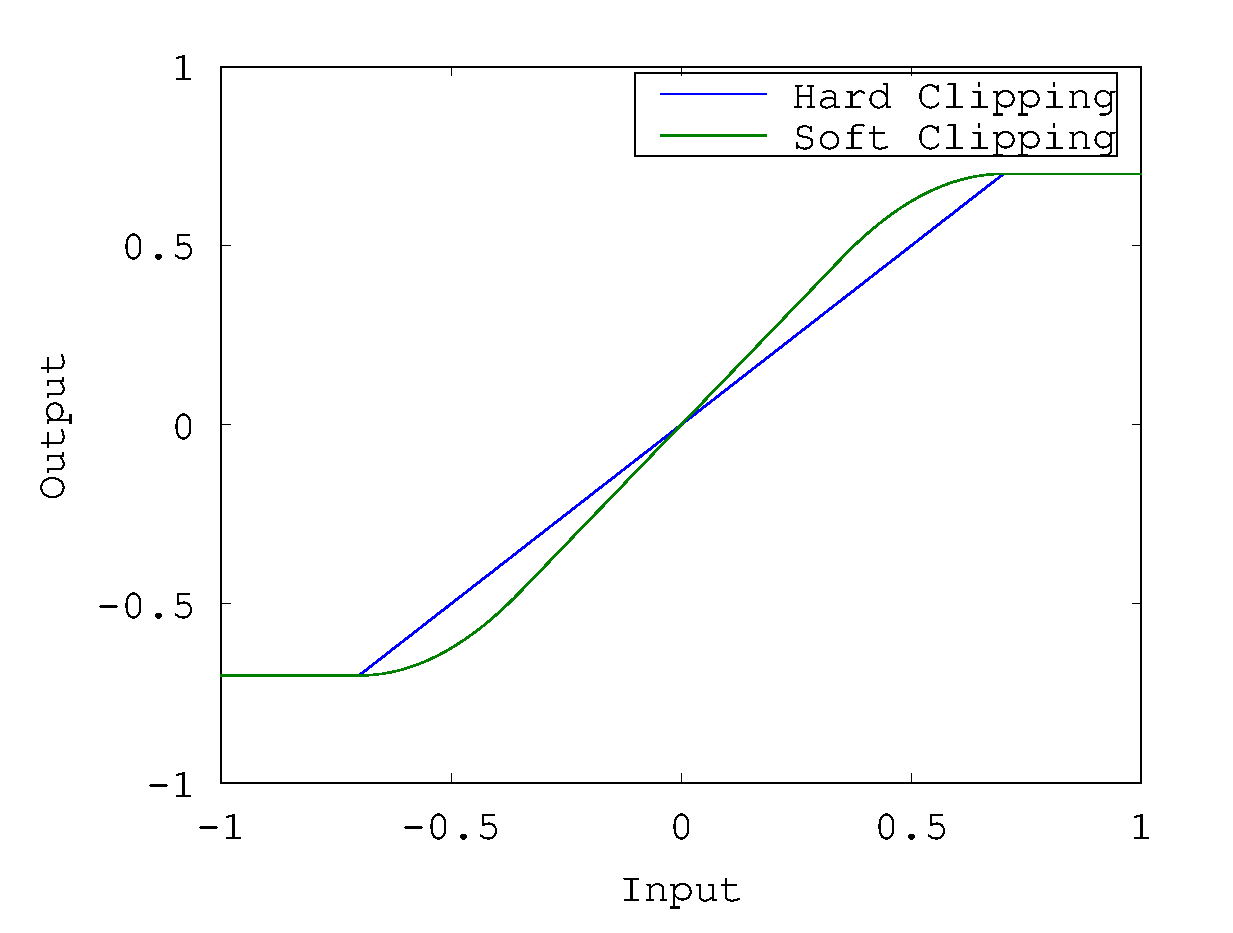
\includegraphics[width=0.6\textwidth]{chapter3/Images/Clipping.eps}
			\caption{Characteristic curves for \ref{eq:SymmetricHardClipping} and
				 \ref{eq:SymmetricSoftClipping} with a threshold of 0.5.}
			\label{fig:Clipping}
		\end{figure}

		\subsubsection*{Complexity}
			Most static nonlinearities only involve a few simple operations for each sample of the input
			signal. The hard clipper from Equation \ref{eq:SymmetricHardClipping} involves only comparisons and
			assignments. A soft clipper could also involve some multiplication and addition.
			
			As each sample is processed individually these algorithms have linear complexity.

		\subsubsection*{Homogeneity}
			The homogeneity of a static nonlinearity depends on the nonlinear function used. For different
			input amplitudes the set of harmonics generated by a given static nonlinearity will change. The
			ways in which this set of harmonics changes was investigated by \citet{enderby2012harmonic}.

			In that study the effects of several soft clippers on sinusoidal inputs were analysed. The levels
			of individual harmonics are plotted as a function of input amplitude. Figures
			\ref{fig:HardClippingHarmonics} and \ref{fig:SoftClippingHarmonics} show these plots for the
			clipping functions described previously.

			\begin{figure}[h!]
				\centering
				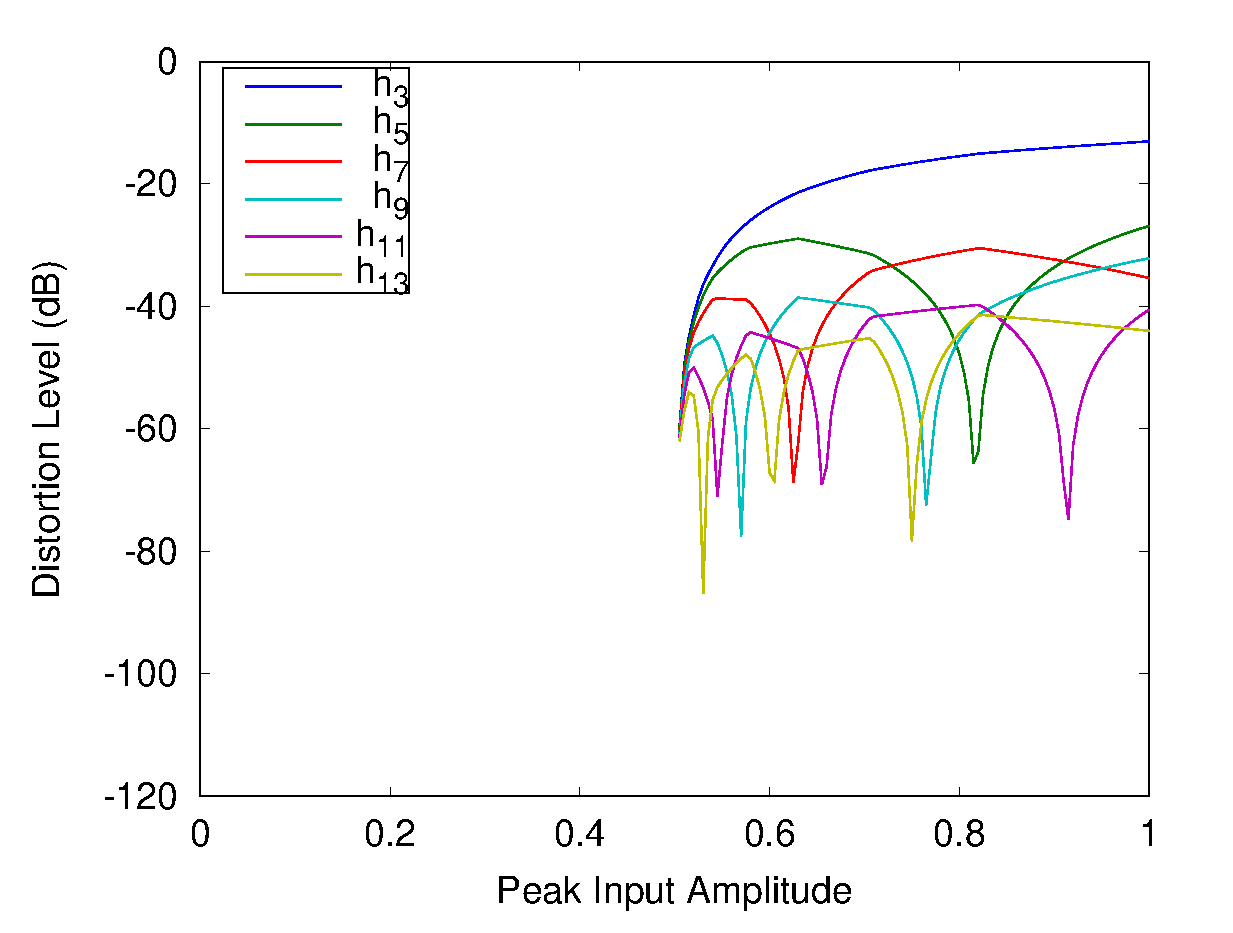
\includegraphics[width=0.6\textwidth]{chapter3/Images/HardClippingHarmonics.eps}
				\caption{Individual harmonic distortion levels for Equation \ref{eq:SymmetricHardClipping}
					 with a threshold of 0.5.}
				\label{fig:HardClippingHarmonics}
			\end{figure}

			\begin{figure}[h!]
				\centering
				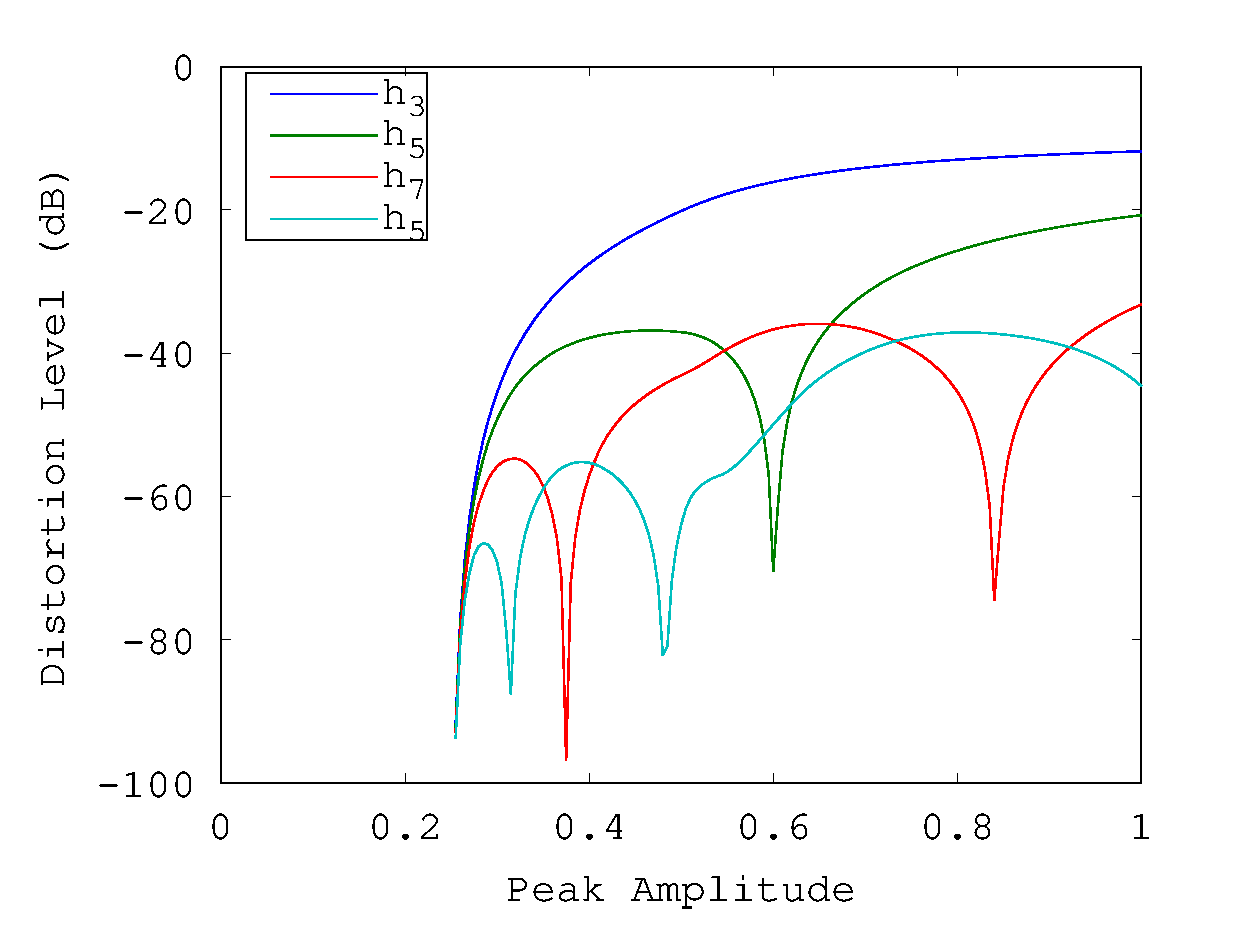
\includegraphics[width=0.6\textwidth]{chapter3/Images/SoftClippingHarmonics.eps}
				\caption{Individual harmonic distortion levels for Equation \ref{eq:SymmetricSoftClipping}
					 with a threshold of 0.5.}
				\label{fig:SoftClippingHarmonics}
			\end{figure}

			The first thing to note is that new harmonic components are only introduced once the input
			amplitude extends out of the linear section of the characteristic curve. Once input amplitude
			reaches a sufficient level harmonics are introduced but their amplitudes all vary independently.

			This behaviour can be improved on through the use of a different clipping function. Equation
			\ref{eq:SymmetricExponentialClipping} shows a function used to apply exponential clipping to a
			signal.
			
			\begin{equation}
				y(n) = \begin{cases}
					t\sgn(x(n)) & \text{if $|x(n)| > t$} \\
					t\sgn(x(n)) \left(1 - \left|\frac{x(n)}{t} - \sgn(x(n)) \right|^{E} \right) &
						\text{otherwise}
				\end{cases}, \quad t \geq 0 \ \text{and} \ E > 1
				\label{eq:SymmetricExponentialClipping}
			\end{equation}

			Where $E$ is a second parameter called the exponent. One advantage of this clipper is that it has
			no linear section. This means that harmonics are generated for input signals of any amplitude.
			Another advantage is that the levels of the generated harmonics vary more uniformly with input
			amplitude as shown in Figure \ref{fig:ExponentialClippingHarmonics}.

			\begin{figure}[h!]
				\centering
				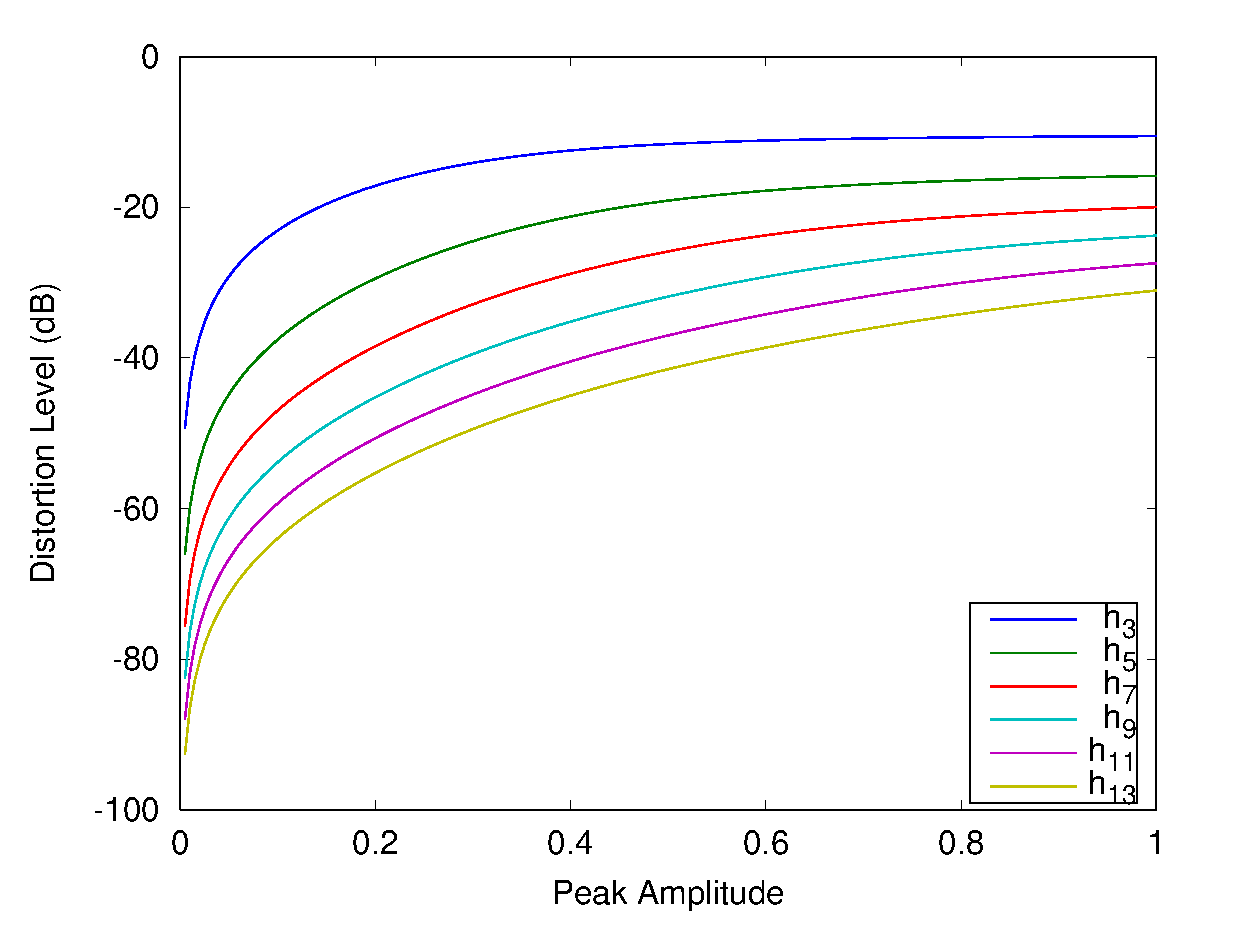
\includegraphics[width=0.6\textwidth]{chapter3/Images/ExponentialClippingHarmonics.eps}
				\caption{Individual harmonic distortion levels for Equation
					 \ref{eq:SymmetricExponentialClipping} with a threshold of 0.5 and an 
				         exponent of 5.}
				\label{fig:ExponentialClippingHarmonics}
			\end{figure}

			The non-homogeneity of simple clipping systems can be counteracted by introducing gain stages either
			side of the clipping stage. The first gain stage scales the signal so that the clipping stage will
			always clip the same proportion of the signal. The second gain stage scales the signal back to the
			original input amplitude. Analogously the clipping function can be scaled so as to always clip the
			same proportion of the signal, as done by \citet{deman2014adaptive}.

		\subsubsection*{Spectral Characteristics}
			The spectral characteristics depend on the function applied to the signal. If an odd function is
			used only odd order intermodulation components will be produced. Using an even function only even
			order components are generated. 

			The symmetric clippers discussed previously all use odd functions. It is evident from the harmonic
			amplitude plots that only odd order harmonics have been introduced to the signal. In order to
			generate even order harmonics these clipping function needs to be made asymmetric. This is easily
			done by clipping negative and positive portions of the input signal at different thresholds.
			Equation \ref{eq:SymmetricHardClipping} can be modified to allow for asymmetric clipping giving
			Equation \ref{eq:AsymmetricHardClipping}.
			
			\begin{equation}
				y(n) = \begin{cases}
					t_{+} & \text{if $x(n) > t_{+}$} \\
					t_{-} & \text{if $x(n) < t_{-}$} \\
					x(n) & \text{otherwise}
				\end{cases}, \quad t_{-} < t_{+}
				\label{eq:AsymmetricHardClipping}
			\end{equation}

			Where $t_{+}$ and $t_{-}$ are the clipping thresholds for positive and negative portions of the
			signal respectively.	

			The amplitudes of the generated harmonics will roll off at differing rates depending on the
			properties of the output signal. The spectrum will roll off at $6(n+1)$dB per octave when the
			$n^{\text{th}}$ derivative of the output signal is discontinuous \citep{kraght2000aliasing}.

			Hard clippers introduce discontinuities to the first derivative of a signal and so will introduce
			harmonics whose amplitudes will roll off at 12dB per octave. Signals clipped by Equation
			\ref{eq:SymmetricSoftClipping} are continuous in the first derivative \todo{(check this)} and so
			produce harmonics which roll off at a faster rate. This can be seen in Figure
			\ref{fig:ClippingSpectra}.

			\begin{figure}[h!]
				\centering
				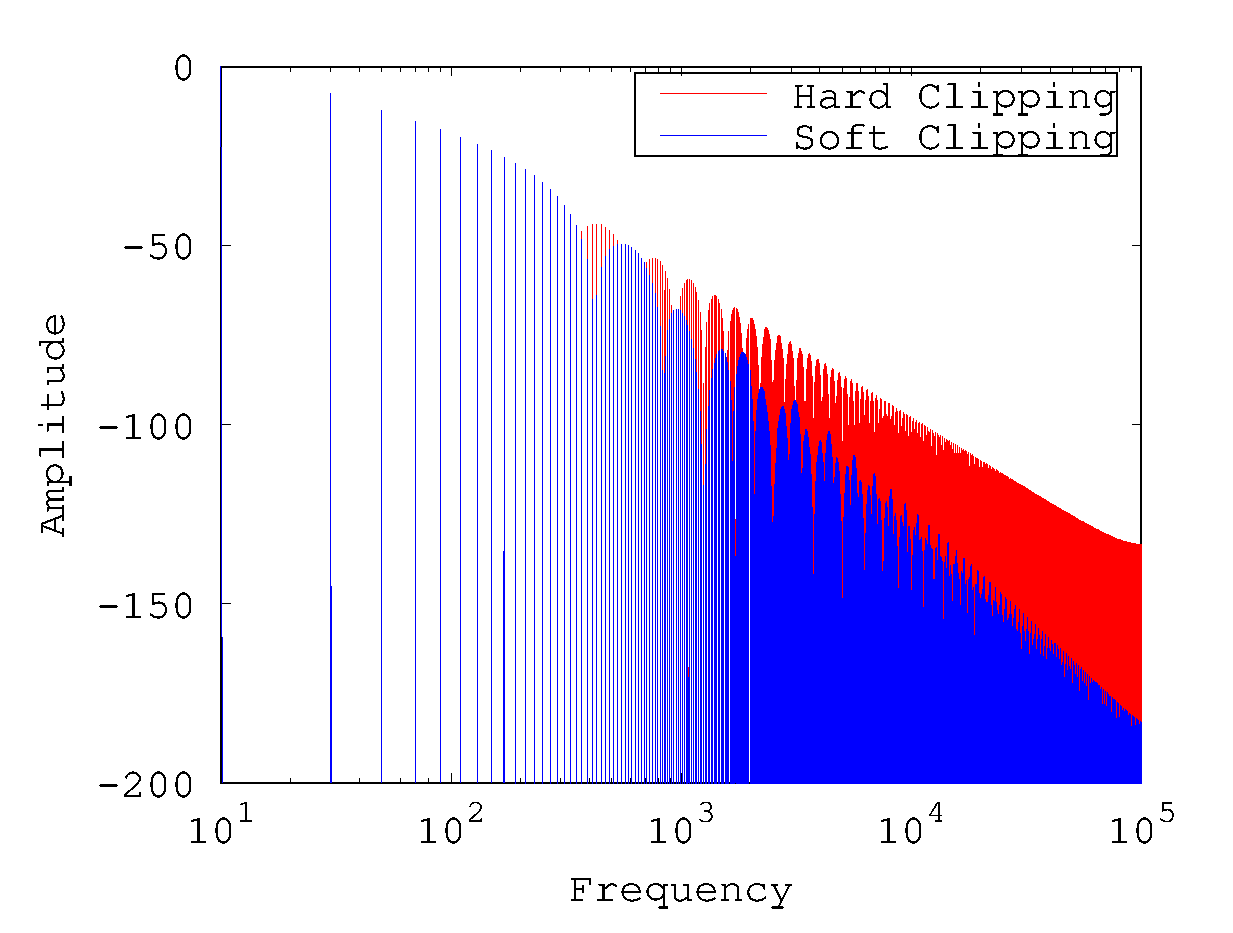
\includegraphics[width=0.6\textwidth]{chapter3/Images/ClippingSpectra.eps}
				\caption{Spectra of sinusoids clipped using Equations \ref{eq:SymmetricHardClipping} and
			                 \ref{eq:SymmetricSoftClipping}.}
				\label{fig:ClippingSpectra}
			\end{figure}

			The steeper roll off produced by soft clippers reduces the number of aliased frequencies produced.
			This is advantageous as aliased frequencies tend to be inharmonic.

		\subsubsection*{Temporal Characteristics}
		\subsubsection*{Flexibility}
		\subsubsection*{Naturalness}

	\subsection{Rectification}
	\label{sec:Excitation-Rectification}
		Rectification is a special case of static nonlinearity. Signals can be either half or full wave rectified,
		as shown in Equations \ref{eq:HalfWaveRectification} and \ref{eq:FullWaveRectification} respectively.

		\begin{equation}
			y(n) = \begin{cases}
				0 & \text{if $x(n) < 0$} \\
				x(n) & \text{otherwise}
			\end{cases}
			\label{eq:HalfWaveRectification}
		\end{equation}

		\begin{equation}
			y(n) = |x(n)|
			\label{eq:FullWaveRectification}
		\end{equation}

		\subsubsection*{Complexity}
		\subsubsection*{Homogeneity}
		\subsubsection*{Spectral Characteristics}
		\subsubsection*{Temporal Characteristics}
		\subsubsection*{Flexibility}
		\subsubsection*{Naturalness}

	\subsection{Integrator}
	\label{sec:Excitation-Integrator}
		Equation \ref{eq:Integrator} shows an Integrator adapted from the one described by \citet{larsen2004audio}.

		\begin{equation}
			y(n) = \begin{cases}
				0 & \text{if $x(n) > 0$ and $x(n - 1) \leq 0$} \\
				y(n - 1) + c|x(n)| & \text{otherwise}
			\end{cases}
			\label{eq:Integrator}
		\end{equation}

		\subsubsection*{Complexity}
		\subsubsection*{Homogeneity}
		\subsubsection*{Spectral Characteristics}
		\subsubsection*{Temporal Characteristics}
		\subsubsection*{Flexibility}
		\subsubsection*{Naturalness}

	\subsection{Multiplier}
	\label{sec:Excitation-Multiplier}
		\begin{equation}
			y(n) = x(n)^{h}, \quad h \in \mathbb{N}
			\label{eq:Multiplier}
		\end{equation}

		\subsubsection*{Complexity}
		\subsubsection*{Homogeneity}
		\subsubsection*{Spectral Characteristics}
		\subsubsection*{Temporal Characteristics}
		\subsubsection*{Flexibility}
		\subsubsection*{Naturalness}

	\subsection{Single Side Band Automodulation}
	\label{sec:Excitation-SSB}
		Single sideband automodulation utilises the concept of single sideband modulation
		\citep{corinthios2009signals}. This allows you to apply amplitude modulation to a signal and only produce
		either the sum or difference sideband.

		A simple way to apply single sideband modulation to a signal is through construction of an analytic signal.
		An analytic signal is a complex valued signal, the real part of which is the original signal and the
		imaginary part its Hilbert transform. The analytic signal is often denoted with a subscript letter
		$a$, such that the analytic representation of the signal $x(n)$ would be denoted $x_{a}(n)$.

		\note
		{
			We probably need some place to talk about hilbert transforms \citet{oppenheim2014discrete} are
			pretty good at that shiz.
		}

		In single sideband automodulation the analytical representation of the input signal is multiplied with
		itself in order to generate harmonics. Equation \ref{eq:SSB} shows the $h^{\text{th}}$ order single side
		band automodulation of a signal.

		\begin{equation}
			y(n) = \Re \left( x_{a}(n)^{h} \right), \quad h \in \mathbb{N}
			\label{eq:SSB}
		\end{equation}

		\subsubsection*{Complexity}
		\subsubsection*{Homogeneity}
		\subsubsection*{Spectral Characteristics}
		\subsubsection*{Temporal Characteristics}
		\subsubsection*{Flexibility}
		\subsubsection*{Naturalness}

	\subsection{Instantaneous Amplitude and Phase}
	\label{sec:Excitation-IAP}
		In this method, the instantaneous amplitude and phase of the analytic signal are calculated. These values
		are then used to aid in the construction of harmonics. The instantaneous amplitude of the analytic signal
		is found by taking its absolute value, $|x_{a}(n)|$. The instantaneous phase is found by taking the complex
		argument of the analytic signal, $\arg(x_{a}(n))$. The instantaneous phase can then be scaled in order to
		scale the frequency content of the signal independent of its amplitude. Equation \ref{eq:IAP} shows the
		$h^{\text{th}}$ order instantaneous amplitude and phase modulation of a signal.

		\begin{equation}
			y(n) = |x_{a}(n)| \cos \left( h\arg(x_{a}(n)) \right), \quad h \in \mathbb{N}
			\label{eq:IAP}
		\end{equation}

		\subsubsection*{Complexity}
		\subsubsection*{Homogeneity}
		\subsubsection*{Spectral Characteristics}
		\subsubsection*{Temporal Characteristics}
		\subsubsection*{Flexibility}
		\subsubsection*{Naturalness}

	\subsection{Spectral Replication}
	\label{sec:Excitation-SpectralReplication}
		The principle behind spectral replication is to reproduce the spectral structure of a signal at higher
		frequencies.

		\begin{figure}[h!]
			\centering
			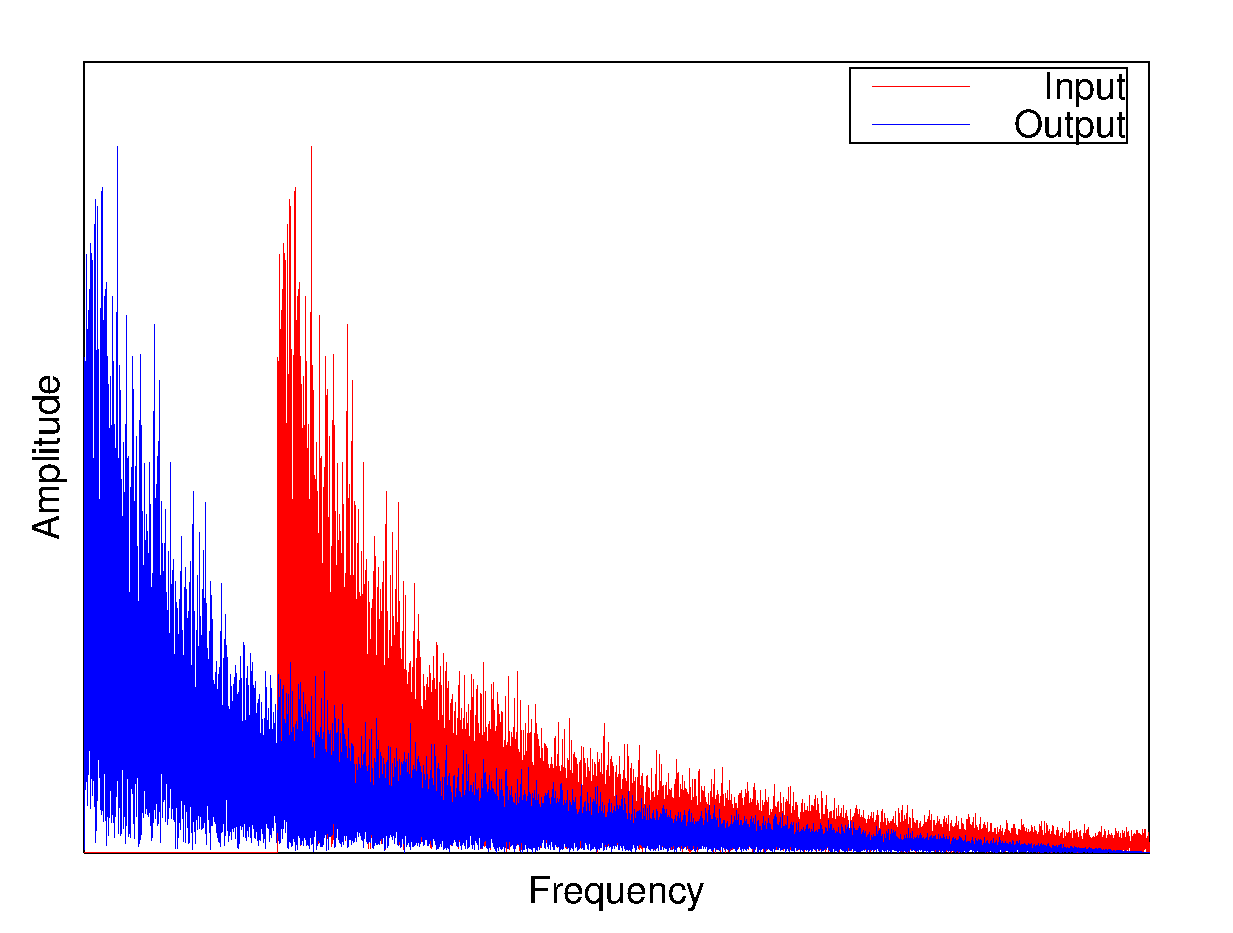
\includegraphics[width=0.6\textwidth]{chapter3/Images/SpectralReplicationSpectrum.eps}
			\caption{The spectral characteristics of spectral replication.}
			\label{fig:SpectralReplication}
		\end{figure}

		This spectral shift is easily implemented through the use of single side band modulation as shown in
		Equation \ref{eq:SpectralReplication}.

		\begin{equation}
			y(n) = \Re \left( x_{a}(n) e^{j\omega  n/ f_{s}} \right)
			\label{eq:SpectralReplication}
		\end{equation}

		Where $\omega$ is the angular frequency the signal should be shifted by and $f_{s}$ is the sampling
		frequency of the signal.

		\subsubsection*{Complexity}
		\subsubsection*{Homogeneity}
		\subsubsection*{Spectral Characteristics}
		\subsubsection*{Temporal Characteristics}
		\subsubsection*{Flexibility}
		\subsubsection*{Naturalness}

	\subsection{Spectral Folding}
	\label{sec:Excitation-SpectralFolding}
	
		\begin{figure}[h!]
			\centering
			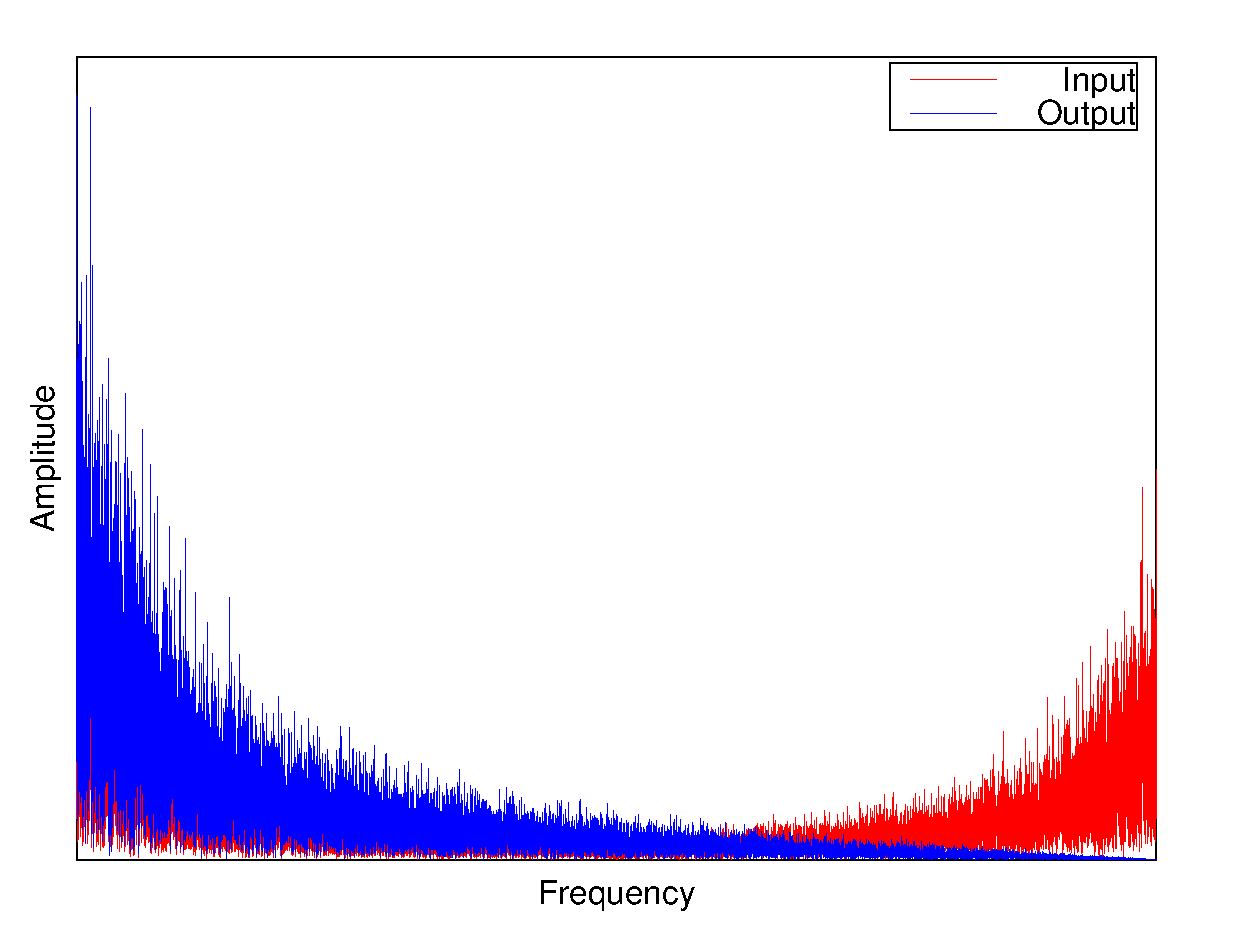
\includegraphics[width=0.6\textwidth]{chapter3/Images/SpectralFoldingSpectrum.eps}
			\caption{The spectral characteristics of spectral folding.}
			\label{fig:SpectralFolding}
		\end{figure}

		\begin{equation}
			y(n) = \begin{cases}
				-x(n) & \text{if $n$ is odd} \\
				x(n) & \text{otherwise}
			\end{cases}
			\label{eq:SpectralFolding}
		\end{equation}

		\subsubsection*{Complexity}
		\subsubsection*{Homogeneity}
		\subsubsection*{Spectral Characteristics}
		\subsubsection*{Temporal Characteristics}
		\subsubsection*{Flexibility}
		\subsubsection*{Naturalness}

	\subsection{Spectral Stretching}
	\label{sec:Excitation-SpectralStretching}

		\begin{figure}[h!]
			\centering
			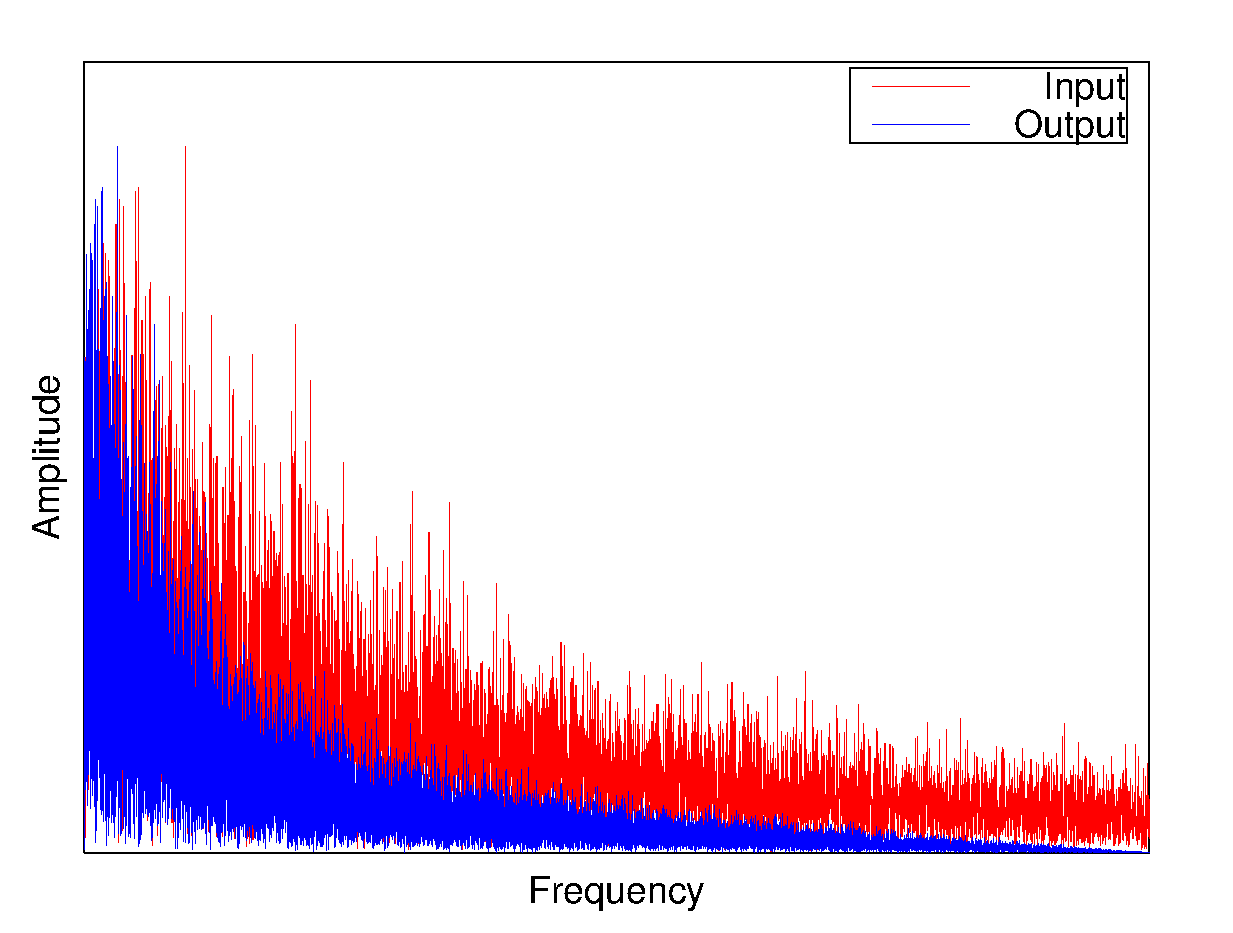
\includegraphics[width=0.6\textwidth]{chapter3/Images/SpectralStretchingSpectrum.eps}
			\caption{The spectral characteristics of spectral stretching.}
			\label{fig:SpectralStretching}
		\end{figure}

		\subsubsection*{Complexity}
		\subsubsection*{Homogeneity}
		\subsubsection*{Spectral Characteristics}
		\subsubsection*{Temporal Characteristics}
		\subsubsection*{Flexibility}
		\subsubsection*{Naturalness}

	%\subsection{Bandwidth Extension}
	%\label{sec:Excitation-BWE}
	%	\note
	%	{
	%		A nice summary in \citet{larsen2004audio}.

	%		Look at Figure \ref{fig:SpectralFolding} 'aint it fancy.
	%	}

	%	\begin{figure}[h!]
	%		\centering
	%		\subfloat[Spectral Folding]
	%		{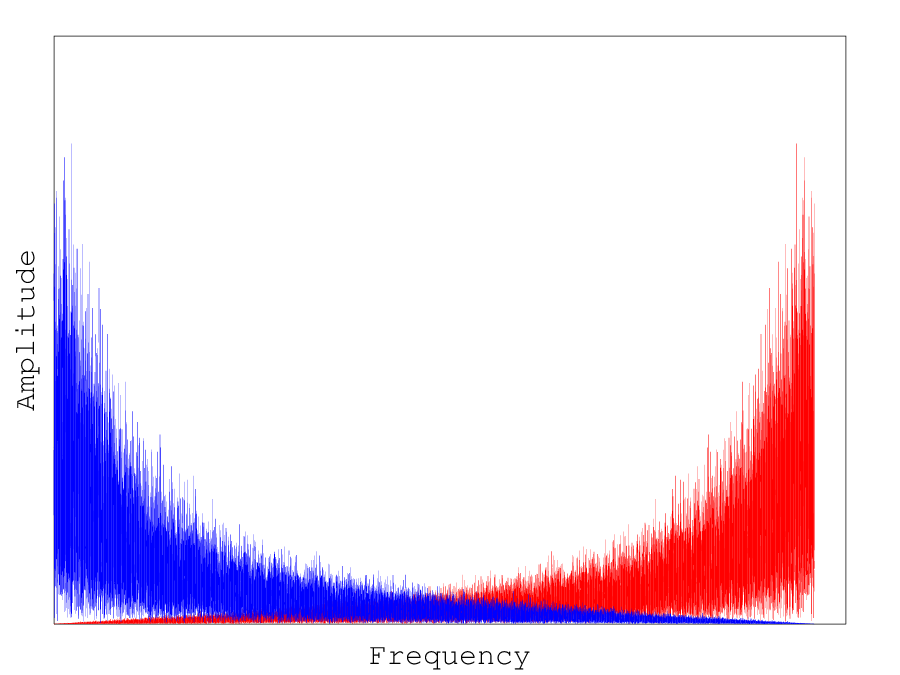
\includegraphics[width=0.4\textwidth]{chapter3/Images/SpectralFolding.png}}
	%		\subfloat[Spectral Replication]
	%		{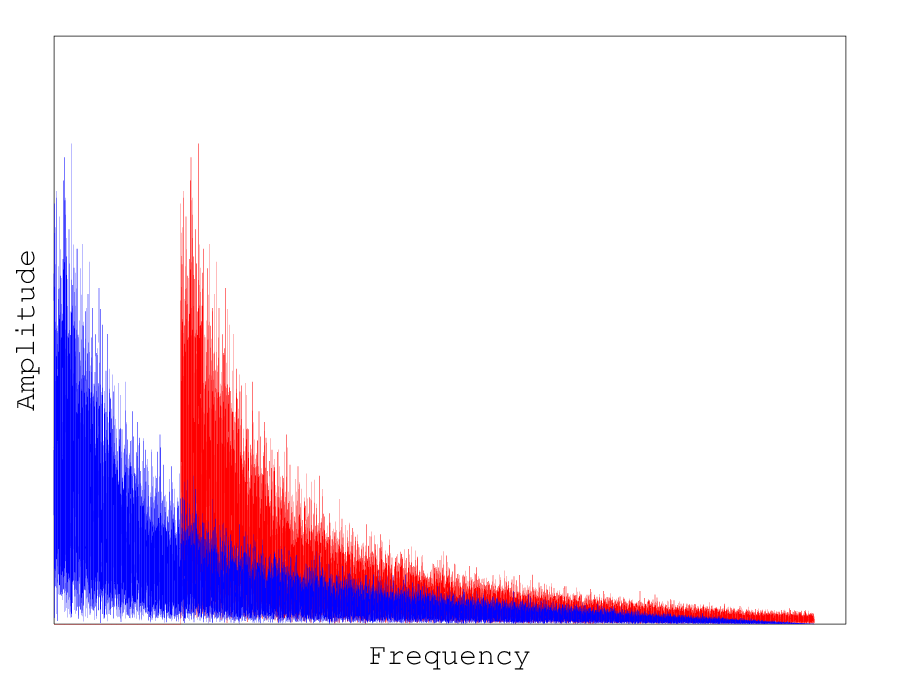
\includegraphics[width=0.4\textwidth]{chapter3/Images/SpectralReplication.png}}
	%		\\
	%		\subfloat[Spectral Stretching]
	%		{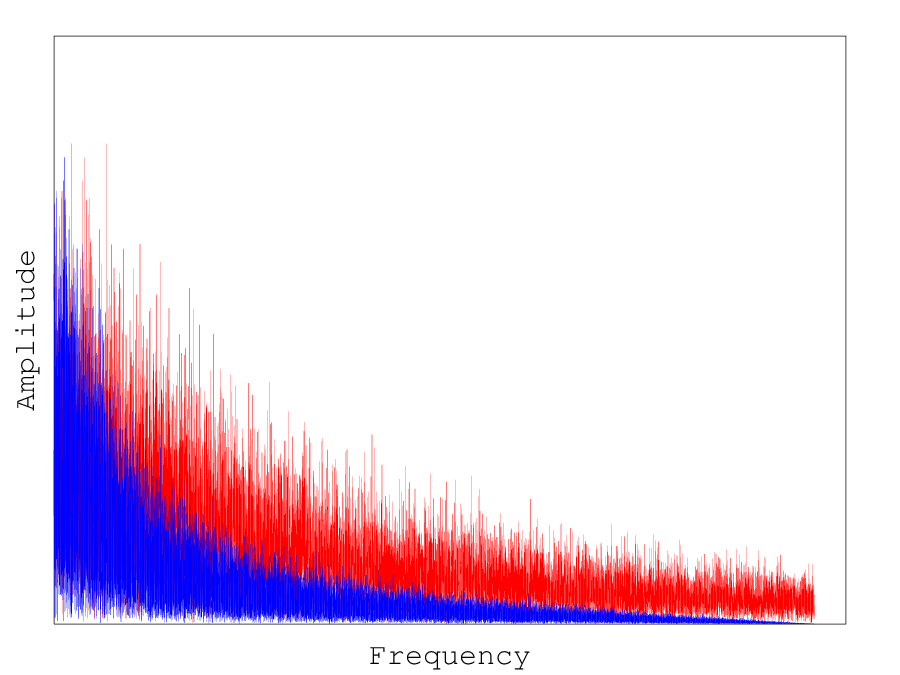
\includegraphics[width=0.4\textwidth]{chapter3/Images/SpectralStretching.png}}
	%		\caption{Spectral characteristics of different band width extension methods. In each graph the blue 
	%		section represents the original spectra and the red section the new spectral content.}
	%		\label{fig:SpectralFolding}
	%	\end{figure}

	\subsection{Individual Harmonic Generation}
	\label{sec:Excitation-Individuals}
		\note{SMC paper}

	\subsection{Psychoacoustic Enhancers}
	\label{sec:Excitation-Enhancers}
		\note
		{
			Probably the most well known perceptual control effects out there. The Aural Exciter has been 
			covered by both \citet{chalupper2000aural} and \citet{shekar2013modeling}.
		}

	\subsection{Fundamental Frequency Tracking}
	\label{sec:Excitation-Fundamental}
		\note
		{
			Several generation methods can be improved through tracking the fundamental frequency of the input 
			signal.

			We can talk all about fundamental / pitch tracking here \citep{cuadra2001efficient, 
			gerhard2003pitch, prukkanon2009vt-amdf, larsen2004audio}.
		}

\begin{landscape}
\section{Methods Comparison}
\label{sec:Excitation-Comparison}

	\begin{tabular}{|c|c|c|c|c|c|c|}
		\hline
		\bf{Method} & \bf{Complexity} & \bf{Homogeneity} & \bf{Spectral Properties} & \bf{Temporal Properties} & \bf{IMD}
		\bf{Flexibility} & \bf{Naturalness} \\
		\hline
		Static Nonlinearity & $\mathcal{O}(n)$ & & & & & \\
		\hline
		Rectifier & $\mathcal{O}(n)$ & & & & & \\
		\hline
		Integrator & $\mathcal{O}(n)$ & & & & & \\
		\hline
		Multiplier & $\mathcal{O}(n)$ & & & & & \\
		\hline
		SSB & $\mathcal{O}(n)$ & & & & & \\
		\hline
		IAP & $\mathcal{O}(n)$ & & & & & \\
		\hline
		Spectral Replicator & $\mathcal{O}(n)$ & & & & & \\
		\hline
		Spectral Mirror & $\mathcal{O}(n)$ & & & & & \\
		\hline
		Spectral Stretch & $\mathcal{O}(n\log{n})$ Assuming FFT used & & & & & \\
		\hline
	\end{tabular}

\end{landscape}

%\section{Evaluating Excitation Methods}
%\label{sec:FeatureControl-MethodEvaluation}
%
%	\note{Homogeneity a la DAFx paper.
%	      Flexibility introduced by allowing single harmonic control a la SMC paper}
%
%	Several harmonic excitation methods were discussed in Section \ref{sec:Excitation-Methods}. When applied to the 
%	task of controlling specific audio features each of these methods has its own advantages and disadvantages.
%
%	\subsection{Homogeneity}
%	\label{sec:FeatureControl-Homogeneity}
%
%		\subsubsection*{Static Nonlinearities}		
%			As previously mentioned simple static nonlinearities are very susceptible to change in input 
%			amplitude. \citet{deman2014adaptive} counteract this issue by having the clipping threshold adapt 
%			to changes in the RMS amplitude of the input. The user is then provided with a `relative threshold' 
%			parameter on which the same setting should give similar perceptual results no matter what the input 
%			amplitude.
%
%			\note{Talk about the issues with static nonlinearities raised in \citet{enderby2012harmonic}}
%
%		\subsubsection*{Bandwidth Extension}
%			\note{Spectral mirroring, stretching and replication are all homogeneous.}
%			
%		\subsubsection*{Single Harmonic Generation}
%			Using single sideband automodulation the proportion of new frequency components in the output 
%			signal increases as the input amplitude increases. The instantaneous amplitude and phase and phase 
%			vocoder techniques are more robust in this respect.
%
%	\subsection{Flexibility}
%	\label{sec:FeatureControl-Flexibility}
%
%		\note{Flexibility is provided by individual harmonic generation \citep{enderby2013methods}}	
%
%	\subsection{Complexity}
%	\label{sec:FeatureControl-Complexity}
%		
%		\note{It is advantageous to use an algorithm that will create accurate harmonics with little analysis.
%		      Most methods don't rely on knowing the fundamental in order to generate harmonics. Spectral
%		      shifting on the other hand does.}
%
%		\note{Most of the algorithms can be easily improved through the use of a low pass filter, increasing
%	             complexity.}
